\documentclass{beamer}
% \usepackage[utf8]{inputenc}

\usepackage{amsmath, amsfonts, amssymb}
\usepackage{amsthm}
\usepackage{mathtools}
\usepackage{physics}
\usepackage[super]{nth}

\usepackage{graphicx}
\graphicspath{{../assets/}}

\usepackage{pgfplots}
\usepackage{tikz}
\usepackage{standalone}

\newcommand{\ee}{\operatorname{e}}          % Euler's number
\newcommand{\ii}{\mathrm{i}}                % imaginary unit
\newcommand{\ad}[1]{a_{#1}^{\dagger}}       % creation operator
\newcommand*\mean[1]{\overline{#1}}         % mean

\usetheme{metropolis}           % Use metropolis theme
\title{Large-Scale Numerical Investigations into the Dynamics of Nonlinear Classical Systems}
\date{\today}
\author{Sebastian Micluța-Câmpeanu}
\institute{University of Bucharest}
\begin{document}
\maketitle

%%%%%%%%%%%%%%%%%%%%%%%%%%%% slide 1 %%%%%%%%%%%%%%%%%%%%%%%%%%%%

\begin{frame}{Outline}
  \tableofcontents[]
\end{frame}

%%%%%%%%%%%%%%%%%%%%%%%%%%%% slide 2 %%%%%%%%%%%%%%%%%%%%%%%%%%%%

\begin{frame}{Acknowledgements}
	\begin{itemize}
		\item I would like to thank A.I.~Nicolin, and V.~Băran for helping and motivating me.
		\item The author has been	supported by PN-III-P4-ID-PCE-2016-0792.
		\item All numerical simulations were performed on the computing cluster of
		Department of Computational Physics and Information Technologies,
		``Horia Hulubei'' National Institute for Physics and Nuclear Engineering.
	\end{itemize}
\end{frame}

\section{Introduction}

%%%%%%%%%%%%%%%%%%%%%%%%%%%% slide 3 %%%%%%%%%%%%%%%%%%%%%%%%%%%%

\begin{frame}{The model}
  \begin{itemize}
		\item The physical system that we model is the surface of heavy nuclei.
    \item The Hamiltonian describes the constrained motion of the vibrational quadrupole degrees of freedom of nuclear surface.
  \end{itemize}
\end{frame}

%%%%%%%%%%%%%%%%%%%%%%%%%%%% slide 4 %%%%%%%%%%%%%%%%%%%%%%%%%%%%

\begin{frame}{The model}
	The Hamiltonian of the system
	\begin{equation*}
    H = \alert<1,2>{\frac{A}{2}\left(p_0^2+p_2^2\right)+\frac{A}{2}\left(q_0^2+q_2^2\right)}
		 +\alert<3>{\frac{B}{\sqrt{2}}q_0\left(3q_2^2-q_0^2\right)}
		 +\alert<2>{\frac{D}{4}\left(q_0^2+q_2^2\right)^2}
  \end{equation*}

	\begin{columns}
		\column{0.5\textwidth}
		\begin{itemize}
			\item \alert<1> {Harmonic oscillator part}
			\item \alert<2> {Integrable part}
			\item \alert<3> {Non-integrable term}
		\end{itemize}

		\column{0.5\textwidth}
		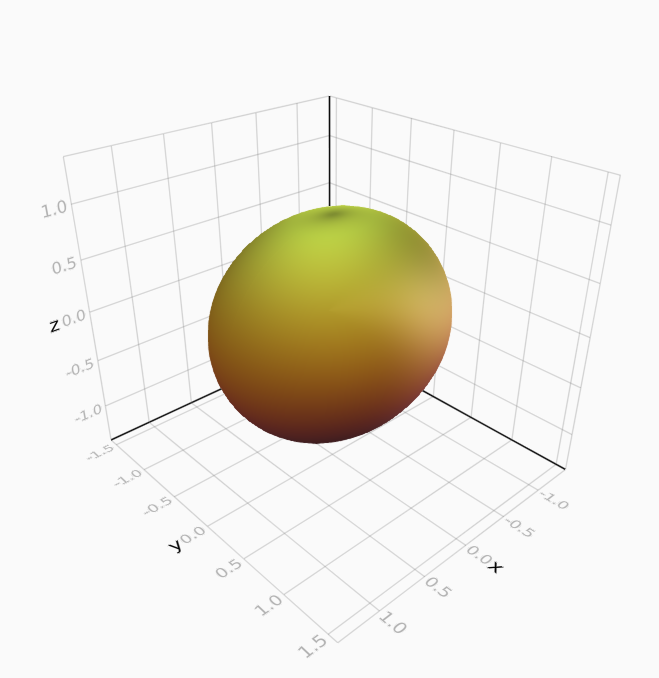
\includegraphics[width=\textwidth]{nucleus}
	\end{columns}
\end{frame}

%%%%%%%%%%%%%%%%%%%%%%%%%%%% slide 5 %%%%%%%%%%%%%%%%%%%%%%%%%%%%


\begin{frame}
	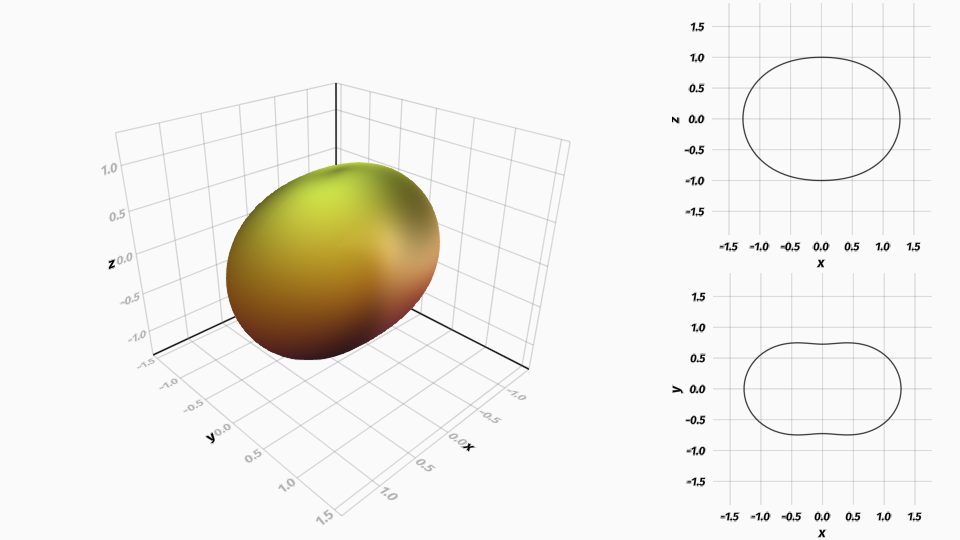
\includegraphics[width=\textwidth]{nucleus-with-sections}
\end{frame}

%%%%%%%%%%%%%%%%%%%%%%%%%%%% slide 6 %%%%%%%%%%%%%%%%%%%%%%%%%%%%

\begin{frame}
	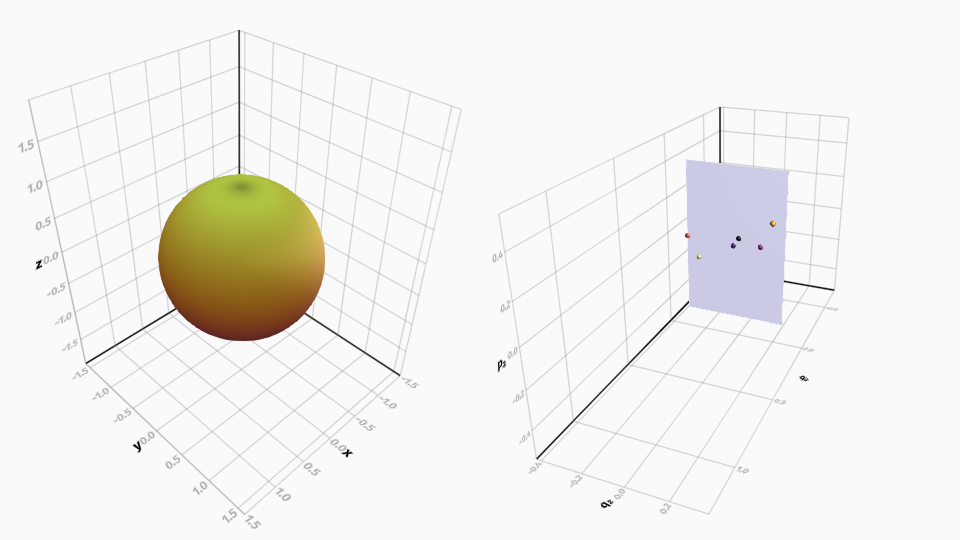
\includegraphics[width=\textwidth]{nucleus-with-poincare}
\end{frame}

\section{Numerical simulations}

%%%%%%%%%%%%%%%%%%%%%%%%%%%% slide 7 %%%%%%%%%%%%%%%%%%%%%%%%%%%%

\begin{frame}
	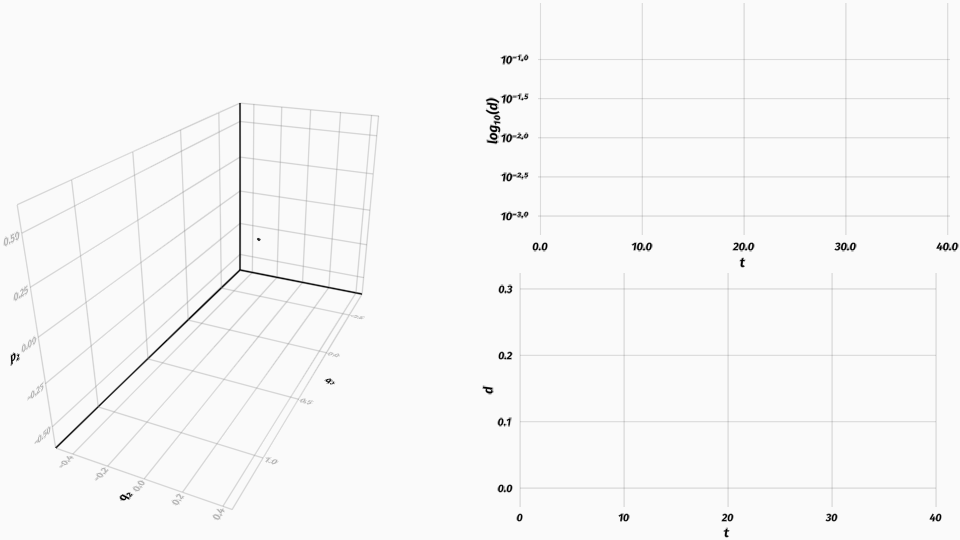
\includegraphics[width=\textwidth]{dist-with-log}
\end{frame}

%%%%%%%%%%%%%%%%%%%%%%%%%%%% slide 8 %%%%%%%%%%%%%%%%%%%%%%%%%%%%

\begin{frame}
	% \includegraphics[width=\textwidth]{poincare-explorer}
\end{frame}

%%%%%%%%%%%%%%%%%%%%%%%%%%%% slide 9 %%%%%%%%%%%%%%%%%%%%%%%%%%%%

\begin{frame}
	\begin{figure}
		\includestandalone[width=\textwidth]{../assets/short-benchmark-E}
		\caption{Energy error benchmark for short integration time}
	\end{figure}
\end{frame}

%%%%%%%%%%%%%%%%%%%%%%%%%%%% slide 10 %%%%%%%%%%%%%%%%%%%%%%%%%%%%

\begin{frame}
	\begin{figure}
		\includestandalone[width=\textwidth]{../assets/short-benchmark-t}
		\caption{Computational time benchmark for short integration time}
	\end{figure}
\end{frame}

%%%%%%%%%%%%%%%%%%%%%%%%%%%% slide 11 %%%%%%%%%%%%%%%%%%%%%%%%%%%%

\begin{frame}
	\begin{figure}
		\includestandalone[width=\textwidth]{../assets/short-benchmark-rescaling-E}
		\caption{Energy error benchmark for short integration time with rescaling}
	\end{figure}
\end{frame}

%%%%%%%%%%%%%%%%%%%%%%%%%%%% slide 12 %%%%%%%%%%%%%%%%%%%%%%%%%%%%

\begin{frame}
	\begin{figure}
		\includestandalone[width=\textwidth]{../assets/short-benchmark-rescaling-t}
		\caption{Computational time benchmark for short integration time with rescaling}
	\end{figure}
\end{frame}

%%%%%%%%%%%%%%%%%%%%%%%%%%%% slide 13 %%%%%%%%%%%%%%%%%%%%%%%%%%%%

\begin{frame}
	\begin{figure}
		\includestandalone[width=\textwidth]{../assets/long-benchmark-E}
		\caption{Energy error benchmark for long integration time}
	\end{figure}
\end{frame}

%%%%%%%%%%%%%%%%%%%%%%%%%%%% slide 14 %%%%%%%%%%%%%%%%%%%%%%%%%%%%

\begin{frame}
	\begin{figure}
		\includestandalone[width=\textwidth]{../assets/long-benchmark-t}
		\caption{Computational time benchmark for long integration time}
	\end{figure}
\end{frame}

%%%%%%%%%%%%%%%%%%%%%%%%%%%% slide 15 %%%%%%%%%%%%%%%%%%%%%%%%%%%%

\begin{frame}
	\begin{figure}
		\includestandalone[width=\textwidth]{../assets/long-benchmark-rescaling-E}
		\caption{Energy error benchmark for long integration time with rescaling}
	\end{figure}
\end{frame}

%%%%%%%%%%%%%%%%%%%%%%%%%%%% slide 16 %%%%%%%%%%%%%%%%%%%%%%%%%%%%

\begin{frame}
	\begin{figure}
		\includestandalone[width=\textwidth]{../assets/long-benchmark-rescaling-t}
		\caption{Computational time benchmark for long integration time with rescaling}
	\end{figure}
\end{frame}

%%%%%%%%%%%%%%%%%%%%%%%%%%%% slide 17 %%%%%%%%%%%%%%%%%%%%%%%%%%%%

\begin{frame}
	\begin{figure}
		\includestandalone[width=\textwidth]{../assets/long-benchmark-rescaling-t}
		\caption{Computational time benchmark for long integration time with rescaling}
	\end{figure}
\end{frame}

\section{Conclusions}

\begin{frame}[standout]
Thank you!
\end{frame}

\end{document}
